%==============================================Intro===========================

% This paper takes a first step towards understanding what network support is required for resource disaggregation. Rather than approach the question from a clean-slate, we adopt a workload-driven approach: we take five diverse workloads commonly found in today's datacenters -- batch processing jobs in Hadoop, point queries with memcached~\cite{memcached}, graph processing with Graphlab -- and address three questions in the context of these workloads: 
%through a combination of emulations and simulation: 

% \cut{
% \vspace{-0.5em}
% \begin{itemize}[leftmargin=*]
% 	\itemsep0em
% 	\item What network latency and bandwidth are required to avoid significantly degrading application-level performance relative to server-centric architectures? 
% 	\item How (and why) does disaggregation change network traffic characteristics such as flow size distributions, communication patterns, traffic volumes, burstiness, and so forth?
%     \item Can existing transport protocols meet the above requirements? 
% \end{itemize}
% }

% \vspace{0.1in}
% \noindent {\bf (1) Network performance requirements:} What network latency and bandwidth are required to avoid degrading application-level performance relative to server-centric architectures? 

% \vspace{0.1in}
% \noindent {\bf (2) Traffic workloads:} How (and why) does disaggregation change network traffic characteristics such as flow size distributions, communication patterns, traffic volumes, burstiness, and so forth?

% \vspace{0.1in}
% \noindent {\bf (3) L3/L4 protocols:} Can existing (deployed or proposed) network designs meet the above requirements?


% \cut{ 
% %SR: need to find a place to discuss this (but not here)
% To date, there is no consensus on the granularity at which resource disaggregation will happen --- at the rack-scale, pod-scale, or an extreme of datacenter scale. Moreover, as briefly discussed above, resource disaggregation enables flexibility in choice of provisioning and sharing of resources adding to the degrees of freedom in design of \dis architecture. Given that our focus is on understanding the network support for \dis (rather than proposing a \dis architecture), we consider the new degrees of freedom --- scale of disaggregation, CPU-memory disaggregation, data placement and access, etc. --- as design parameters that may impact our study. 
% } 

% \vspace{0.5em}
% \noindent Our key findings are as follows:
% \vspace{-0.5em}
% \begin{itemize}[leftmargin=*]
% \itemsep0em
% 	\item To maintain application performance comparable to current datacenters, a disaggregated datacenter must provide at least $40$Gbps bandwidth to end-points and an end-to-end latency of no more than $5-10\mu$s.
% 	\item Traffic workloads in a disaggregated datacenter will differ significantly from existing workloads. Specifically, we observe: (a) up to 85\% less skew in flow size distributions, (b) a 100x reduction in the size of the longest (`elephant') flows, (c) up to a $75\times$ increase in overall traffic volume, and (d) a more uniform temporal distribution of traffic.
% 	\item 
	
% \end{itemize} 
	


% \cut{
% \noindent
% \sr{Add a list of caveats/disclaimers as follows\ldots}
% \begin{itemize} 
% \item our results are based on the workloads we study; not comprehensive
% \item we focus on net design, ignore many systems questions; may still well turn out that the latter matters more; in this sense one might view our study as seeing whether the network can `get out of the way’ \cite{};
% \item because our study is forward looking, many aspects of the overall context we’re considering don’t exist yet so we must make assumptions - e.g., data layout, how resources blades are organized, etc.  We 
% \end{itemize} 
% }






%=======================================summary===============================
\cut{ 
In this section, we discuss existing disag
gregated hardware prototypes (\S\ref{ssec:prototype}), and use the commonalities across these prototypes to motivate the set of assumptions made in our study (\S\ref{ssec:hardware}, \S\ref{ssec:system}).
} 

\cut{ 
that allow us to study the impact of several of the above design aspects on application-level performance in disaggregated datacenters 
} 


\cut{
{\bf Virtual Machine abstraction} to aggregate slices of resources required for computing tasks.
} 


\cut{
	{\bf Specialized Intra-rack network fabric} that use non-commodity components (\eg, Silicon photonics or PCIe links) and protocols, with a clear separation from inter-rack network fabric that comprises of commodity components and legacy protocols.
}
%\end{enumerate}

\cut{
We start by outlining the hardware design we assume for \dis; our assumptions follow previous studies and existing disaggregated prototypes~\cite{ddcHwDesign1, ddcHwDesign2, ddcHwDesign3, rsa, hptm, fdr, sonuma, firebox}. We refer the reader to~\cite{ddcHwDesign1, ddcHwDesign2, ddcHwDesign3} for detailed hardware designs.% for disaggregated blades. 
}

\cut{ 
study complements these prototypes by critically exploring several design aspects (\#1, \#4): (i) the impact of CPU-memory disaggregation on application-level performance; (ii) the bandwidth and latency requirements for maintaining application-level performance compared to traditional server-centric architectures; and in particular, the need for specialized network interconnects; and (iii) the possibility of designing a ``flat'' network architecture for resource disaggregated datacenters with disaggregation at the datacenter scale. 


And as we shall see, our study shows that several assumptions implicit in the design of these early prototypes may not be necessary and that, for current workloads, resource disaggregation can be decoupled with the development of emerging network technologies.

}




%=====================================requirements=======================
%Intuitively, we would expect these applications to observe significant performance degradation on disaggregated hardware due to CPU-memory disaggregation.
%Figure~\ref{fig:latb} shows that this is not necessarily the case, if the network fabric can support $5\mu$s end-to-end latency and $40$Gbps access link bandwidth. 

%the performance degradation that results with nine different latency/bandwidth combinations, given 25\% of memory capacity as local.
%\footnote{The small discrepancies between Figures \ref{fig:impb} and \ref{fig:latb} are due to the small number of runs used in Figure \ref{fig:impb}.} 
% of the measured memory footprint for each workload. 
%We now evaluate the application-level performance for various \dis configurations in terms of end-to-end network latency and access link bandwidth at the end hosts (see Figure~\ref{fig:latb}). 





%The dolphin applications are the ones that observe less than $5\%$ performance degradation (within the application performance variance) with a network of $5\mu$s end-to-end latency and $40$Gbps access link bandwidth. 
%Intuitively, the dolphin applications are the ones that are either not optimized to use available memory aggressively (Hadoop wordcount, Hadoop terasort) or are bottlenecked by network I/O (GraphLab, Memcached). Thus, CPU-memory disaggregation does not lead to significant performance degradation.

%Shark applications, on the other hand, exploit the available memory more aggressively and have stringent latency requirements to be able to maintain the performance similar to existing server-centric architectures. 
%Specifically, the shark applications require $3\mu$s end-to-end latency and $40$Gbps access link bandwidth to achieve negligible performance degradation.

%We examine the discuss the implications (and feasibility) of the end-to-end latency and bandwidth requirements of the dolphin and shark applications in \S\ref{ssec:rtt}. Prior to that, we discuss how various parameters may impact our conclusions.

% We make three observations. First, given a network with $5-10\mu$s end-to-end latency and $40$Gbps access link bandwidth, the application-level performance in \dis is within $5\%$ of that in current server-centric datacenters. 
% Second, as shown in Figure \ref{fig:impl}, fixing bandwidth at 40Gbps, the application performance is sensitive to the increase of end-to-end latency.
% Third, increasing the bandwidth to $100$Gbps, while ensuring $5\mu$s end-to-end network latency further reduces any performance degradation to within $2$--$3\%$ (Figure \ref{fig:impbw}).
% Thus, we conclude that \emph{\dis should aim for an end-to-end network latency and bandwidth of $5-10\mu$s and $40$Gbps respectively.}

%\paragraphb{Impact of local memory size}

% of the available main memory{\footnote{The $100\%$ local CPU cache size corresponds to no CPU-memory disaggregation, as in server-centric architectures.} \rc{Shall we say that we use this as our baseline, rather than application-level performance without SIT, to incorporate SIT overhead. (a+x)/(b+x) problem.}}}. 
%  shows that the application-level performance in \dis is within reasonable bounds (roughly $5$\%) of that in a server-centric architecture as long as the local memory cache is no smaller than $25\%$ of main memory. For larger local cache sizes, performance only improves slowly and for any smaller cache size, the performance degrades significantly. 
% We conclude that \emph{a local memory cache that is sized at $25\%$ of current main memory is sufficient} to maintain reasonable application-level performance in \dis. In what follows, unless stated otherwise, we set the local memory size to this value.




\cut{
We examine the feasibility of achieving zero-queueing in the following sections. 

One might consider two possibilities to optimizing for latency. First, adopting $100$Gbps technology \emph{not} because we need the higher capacity but instead to reduce transmission and queueing times. E.g., in the event of congestion as in our example above, the packet's transmission time overheads would be reduced from $4\mu$s to $1.6\mu$s. 
The other option is to consider limiting the scope of disaggregation, for example, to within a single rack. Somewhat surprisingly, the potential benefits of this appear modest: the primary impact (to latency) of limiting the scope of disaggregation is to reduce the propagation delay but this already only consumes $1\mu$s from our budget.
(Again, this ignores the potential benefits due to reduced congestion in a rack-scale architecture, which we consider in \S\ref{sec:existing}.)

Finally, a key latency component will arise from software overheads 
at the endpoints. Research prototypes in Xen have reported per-page overheads of $2-6\mu$s, depending on the page replacement algorithm~\cite{ddcHwDesign1} while recent work has argued that such overheads can be reduced to sub-microseconds with the integration of NIC functions into the CPU and software optimizations~\cite{lowlatency}. Thus, while there is reason to believe that software overheads can be optimized to fit within our target latency budget, demonstrating this remains an important topic for future exploration.

\paragraphb{Implication \#1:}  The bandwidth requirements for resource disaggregation are within the reach of existing technology. The key enabling factor is a network fabric with low ($\sim 5\mu$s) end-to-end latency.

\vspace{0.1in}
\noindent
%We now discuss the feasibility of a network fabric that provides the above end-to-end latency. Indeed, 
There are two unavoidable contributors to end-to-end network latency --- transmission time for packets in the flow, and propagation delay. \sr{offer evidence??} Given that propagation delays are extremely small in existing datacenters, achieving low end-to-end network latency boils down to minimizing the transmission time for packets in the flow. This has several implications for design of \dis:

\paragraphb{Implication \#2:} Applications running atop \dis must observe little or no queueing delays (that is, no network congestion). 

\vspace{0.1in}
\noindent
The queueing delays observed by flow packets depend heavily on both the network traffic as well as network protocols. We return to evaluating the feasibility of achieving little or no queueing delays in \S\ref{sec:existing}. {motivate via Figure~\ref{fig:impb} and Figure~\ref{fig:impl} $\to$} Note that $100$Gbps links are already available at both switch ports and as server NICs, but are not commonly deployed. Transmission delays dominating the end-to-end network latency have the following implication in the context of \dis:
}

\cut{
\paragraphb{Implication \#3:} While capacity constraints do not impose strict bandwidth requirements, one good reason to consider $100$Gbps links is reducing end-to-end network latency via reduction in transmission time. 

\vspace{0.1in}
\noindent
 Finally, propagation delays having little impact on end-to-end network latency has an interesting implication in \dis design:

\paragraphb{Implication \#4:} Ignoring congestion, the scale of disaggregation (rack-, pod- or datacenter-scale) may have little impact on application-level performance, and disaggregation at the extreme of datacenter-scale may indeed be feasible.
}

\cut{
\vspace{0.1in}
\noindent
We evaluate the application-level performance for rack- and datacenter-scale resource disaggregation in \S\ref{sec:existing}. 
}

% While $100$Gbps network bandwidth does not provide significant benefits over the $40$Gbps case, reducing the latency down to $1\mu$s can lead to applications observing essentially no performance degradation. In the hindsight, this is not surprising given our results from \S\ref{sec:workloads}, where we established that the network traffic volume does not increase significantly in \dis compared to \pdis, and that the network flows are dominated by short (latency-sensitive) memory access flows. \rc{$\gets$ needs more concrete intuition; remote memory faster than local disk; applications heavily pipelined; CPU bottleneck?}

%\paragraphb{Benefits of remote memory}
%First, given sufficient network bandwidth and small network latencies, use of remote memory can drastically improve application performance compared to traditional disk-based swap. Since the working set size is hard to predict in advance, memory tends to be highly over-provisioned in datacenter servers to prevent thrashing. Disaggregated remote memory can reduce this waste by providing an elastic memory capacity pooled at the datacenter scale. 

% \paragraphb{Reducing latency more important than increasing bandwidth}
% Second, low latency is more important than high bandwidth. The $100$Gbps bandwidth did not provide any significant improvement over the $40$Gbps link. In contrast, $10\mu$s round-trip latency causes noticeable performance degradation, as compared to the $1\mu$s case.


%
% \begin{figure}
%   \centering
%     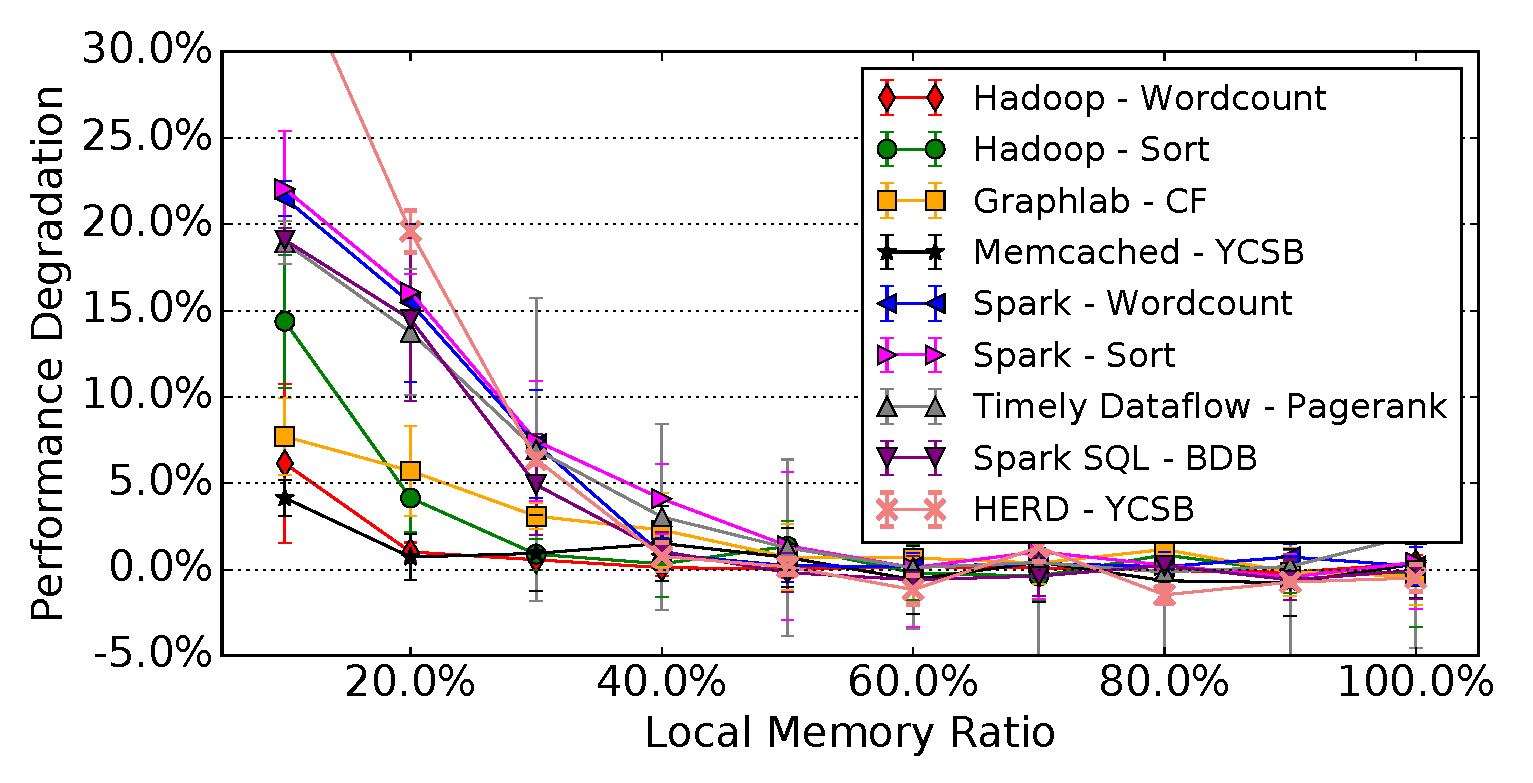
\includegraphics[width = 3.5in]{img/vary_remote_mem.eps} 
%   \caption{\small{\rqc{Fix latency at 5us, bandwidth at 40Gbps, Vary local memory from 0\% to 90\% of the total memory of the EC2 instance}}}
%   \label{fig:impb}
% \end{figure}
%

% graveyard of text scraps.
\cut{
from the network such that the application-level performance in \dis is comparable to that in server-centric architectures.
Overall, our results show that:

\begin{itemize}[leftmargin=*]
	\itemsep0em
	\item CPU blades having local cache is necessary to ensure reasonable performance, given the increased latency to access remote memory. However, $25\%$ of main memory serving as local cache suffices.
	\item Applications require non-trivial latency performance ($5$--$10\mu$s) from the network. In contrast, $40$Gbps access link capacity suffices. Moreover, a good reason to consider higher link capacity is not to handle higher traffic volume, but to reduce the transmission time at the end-hosts.  
    \item Ignoring congestion, the scale of disaggregation (rack versus datacenter scale) has little impact on application-level performance. \rc{$\gets$ right now, we have this results in S5 using simulations for rack and datacenter scale disagg; how should we inject latencies to make this point?}
\end{itemize}

\noindent
}

%Depending on the page eviction algorithm used, 
 %existing research prototypes report this per-page overhead to be roughly in the range of $2$--$6\mu$s~\cite{x1, x2, x3}. However, this overhead can be reduced to sub-microseconds with faster CPUs and software optimization~\cite{y1, y2, y3}, making this overhead insignificant. 











%========================================performance==================

\cut{

We repeat this with the FCTs from our rack-scale simulations. We see that the degradation with datacenter-wide disaggregation is not significantly different from that with rack scale disaggregation. The case with the greatest difference was wordcount, where datacenter- and rack-scale disaggregation incurred 6.2\% and 3.9\% application layer slowdown, respectively. This naturally follows from the results in Figures~\ref{fig:phostp}; since the network layer performance is roughly equal across the two schemes, the application layer performance is as well.
%graphlab: dcscale 4.9 rscale 3.4
}


\cut{ 

Finally, we note that our work su
Note that this contrasts with recent work in the \pdis domain suggesting~\cite{kay-nsdi15} that the network can improve application performance by at most 2\%. Rather, our results suggest that in \dis network-level improvements can have a greater effect.

\paragraphb{Dependent on application characteristics}
The application layer effects depend not only on the network performance as discussed in \S\ref{ssec:nlp} above but also the characteristics of the application being evaluated. For example, memcached and terasort observe similar performance degradation despite memcached having better network performance. 
This is because memcached performs more memory accesses than terasort. 
} 

\cut{
%
\begin{figure*}
  \centering
    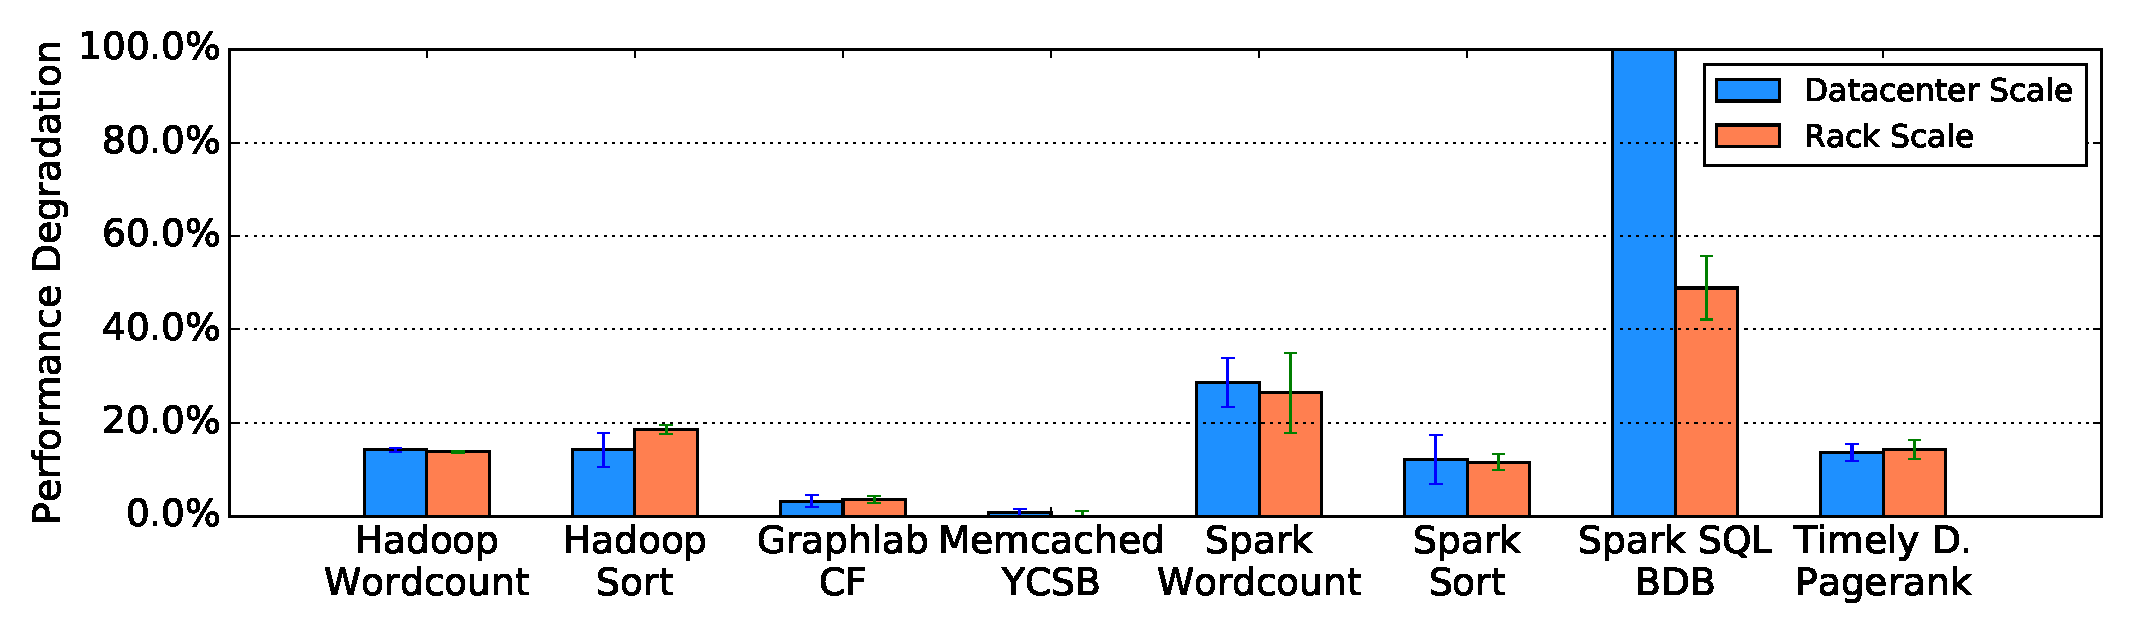
\includegraphics[width = 5in]{img/slowdown40.eps} 
  \caption{\small{Application layer slowdown for each of the four applications at rack-scale and datacenter scale after injecting pFabric's FCT with 40Gbps link. }}
  \label{fig:appfabric40}
\end{figure*}
%
}




%Overall, we conclude that existing protocols should be sufficient to handle disaggregated traffic.

%
% \begin{figure}
% 	\centering
% 	\begin{tikzpicture}[xscale=0.6, yscale=0.35]

% 	\draw[thick, fill=white] (-8, 5) rectangle (-5, 9); 
% 	\draw[thick, fill=white] (-8, 9.75) rectangle (-5, 11.25); 
% 	\draw[thick, fill=white] (-8, 12) rectangle (-5, 14); 
% 	\draw (-6.5, 8.5) node {\small{Network}};
% 	\draw (-6.5, 7.5) node {\small{Simulator}};
% 	\draw (-6.5, 6.5) node {\small{(Individual}};
% 	\draw (-6.5, 5.5) node {\small{Flow delays)}};
% 	\draw (-6.5, 10.5) node {\small{Scale up}};
% 	\draw (-6.5, 13.5) node {\small{Flows from}};
% 	\draw (-6.5, 12.5) node {\small{Step (a)}};
% 	\draw[thick, black, ->] (-6.5, 12) -- (-6.5, 11.25);
% 	\draw[thick, black, ->] (-6.5, 9.75) -- (-6.5, 9);
% 	\draw[thick, black, -] (-5, 7) -- (-4.5, 7);
% 	\draw[thick, black, -] (-4.5, 7) -- (-4.5, 10.5);
% 	\draw[thick, black, ->] (-4.5, 10.5) -- (-3.75, 10.5);

% 	\draw[thick, fill=white] (-3, 5) rectangle (1, 13); 
% 	\draw[thick, fill=white] (-2, 14) rectangle (0, 12); 
% 	\draw (-1, 13) node {\small{CPU}};
% 	% \draw (-1, 10.5) node {\small{Handler}};
	
% 	\draw[thick, fill=cyan] (-3.75, 9.9) rectangle (1.75, 11.1); 
% 	\draw (-1, 10.5) node {\small{SIT (Latency Injection)}};
			
% 	\draw[thick, fill=blue] (-2.75, 7.5) rectangle (-0.75, 8.5);
% 	\draw[thick, fill=green] (-2.75, 5.5) rectangle (-0.75, 7.5);
% 	\draw (-1.75, 8) node {\small{LM}};
% %	\draw (-2.75, 7.5) -- (-0.75, 7.5);
% 	\draw (-1.75, 6.5) node {\small{RM}};
% %	\draw (-2.75, 6.5) -- (-0.75, 6.5);
% %	\draw (-1.75, 6) node {\small{K$\to$O}};

% %	\draw[thick] (-0.25, 5.5) rectangle (0.75, 8.5);
% 	\draw[thick, fill=gray] (-0.25, 8.5) rectangle (0.75, 7.5);
% 	\draw[thick, fill=gray] (-0.25, 5.5) rectangle (0.75, 6.5);
% 	\draw (0.25, 7) node {\small{$\dots$}};

% 	\draw[very thick, black, dashed, <->] (-1.5, 10) -- (-1.75, 8.5);
% 	\draw[very thick, black, dashed, <->] (-0.5, 10) -- (0.25, 8.5);
% 	\draw[very thick, black, dashed, <->] (-0.5, 10) -- (-0.45, 6);

% 	\draw[very thick, black, dashed, <->] (-1.5, 11) -- (-1.5, 12);
% 	\draw[very thick, black, dashed, <->] (-0.5, 11) -- (-0.5, 12);
% 	\draw[very thick, black, dashed, <->] (-0.5, 11) -- (-0.5, 12);

% 	\end{tikzpicture}
% 	    \caption{\small{We run real-world applications on a $5$-node Amazon EC2 cluster. To emulate end-to-end network latency, we inject artificial latencies for all ``remote memory'' and ``remote disk'' accesses and measure the impact of this latency to the application-level performance. The latencies injected for each flow are now a result of network simulation results. \rc{SIT representation imprecise}}}
% 	\label{fig:system3}
% \end{figure}

% \section{To do list:}
% \begin{itemize}
%     \item latency bandwidth requirements argument
%     \item related work
%     \item memcached local mode experiment
%     \item 10G nic experiment (low)
%     \item regenerate fig 8 and 9
%     \item closing loop experiment (fig 10)
    
% \end{itemize}



\cut{
\sr{end v1} 

\sr{start of v2}

To represent a $144$-node topology using only 13 nodes of measurement data (5 CPU, 5 memory, 3 disk as discussed in \S\ref{sec:methol}), we collected two CDFs representing the interarrival and flow size distributions for each of the 70 possible source-destination pairs (recall from the discussion in \S\ref{sssec:spatialdist} that although there are 13 nodes, many source-destination pairs do not communicate).  We then assign each node in the topology a sender profile and 12 other nodes in the destination it will send traffic to. We then generate flows between these chosen source-destination pairs by drawing from the appropriate distribution in our traffic matrix. Overall, this method should approximate network traffic in \dis well enough for our evaluation of transport protocols because it draws from our observed distribution of flows that would appear in \dis.

%\begin{enumerate}
%\item our data is for 5 ec2 nodes, but we have a 144-node topology to fill.
%\item the 5 ec2 nodes map to 5 cpu blades, 5 memory blades, and 3 disk blades
%\item so in our 13-node trace we collect a interarrival and size CDF per s-d pair
%\item for each node in the 144, we assign it a sender profile and pick 12 other nodes as destinations
%\item the interarrival and flow size cdfs for flows between a source and destination as picked in the previous step are used to generate flows.
%\item this should give an idea of network loads in a full-dc disaggregated scenario from a transport perspective.
%\end{enumerate}

%\paragraphb{Level of disaggregation: $3\times$ problem?}
In a \pdis datacenter network, each node represents a collection of 3 resources --- one unit each of CPU, memory, and disk. However in \dis each resource is moved into a separate network node. Applying this transformation naively, one node in the old datacenter would now be spread across three nodes (one for each resource type). As a result, the datacenter as a whole would contain one-third the overall computing resources post-disaggregation. Therefore, to fairly simulate network performance in \dis while representing an equal amount of compute resources we must scale our load up by a factor of 3. We solve this problem by sampling from the size and interarrival distributions discussed above three times per source-destination pair when generating flows in our simulator to represent the presence of three units of computing resource per node.

\sr{end v2}
}




\cut{ 
% SR will incorporate later
\an{should this para be moved to section 3? (throughout our experiments we do not inject disk flows blah blah)}
\paragraphb{Latency Injection for Disk Flows}
Unfortunately, the \texttt{blktrace} tool we use to gather the disk access trace does not \emph{intercept} disk accesses as SIT does for remote memory accesses. As a result, we were unable to inject latency into disk accesses in our experiments. However, our results remain significant because memory accesses are much more sensitive to latency injection than disk accesses. Accordingly, when injecting latency to determine application-level performance we only draw from the performance distribution of memory flows in our simulator.
}

%\begin{enumerate}
%\item blktrace does not intercept, it only logs
%\item we cannot inject latency into disk access
%\item this is okay because a. memory is more latency sensitive anyway 
%\item and b. there are more memory flows than disk flows.
%\item accordingly we only consider the slowdown distribution of memory flows when injecting.
%\end{enumerate}

%\begin{enumerate}
%\item before, one "blade" had 3 resources - cpu, memory, disk
%\item now, each "blade" has only one resource
%\item so, each blade should have 3x of its assigned resource
%\item the flow generation from above is run 3x for each node.
%\end{enumerate}





%================================discussion=======================


\cut{ 
\paragraphb{Specialized Hardware}
While these innovative hardware technologies may unlock future gains in application performance and capabilities, they are complementary rather than necessary for disaggregation.

\paragraphb{Shared Pool Abstraction}
Managing large pools of compute resources will be a challenge for disaggregated datacenters. In this vein cluster managers such as Mesos~\cite{mesos} and resource schedulers such as DRF~\cite{drf} may prove useful in efficiently allocating resources to applications.

\paragraphb{Networks in Disaggregated Datacenters}
R2C2~\cite{r2c2} explores the problem of designing a network stack for rack-scale computers, proposing an interconnect topology for disaggregation at the rack-scale and explore the questions of designing efficient routing and congestion control mechanisms in the context of rack-scale disaggregation.
Our study finds that such efforts at enabling disaggregation at the rack scale with specialized interconnects and protocols \an{are largely unnecessary to achieve application performance.}
} 




\cut{
\paragraphb{Research prototypes} \rc{Remove? Already discussed in S2 $\to$} Rack-scale disaggregation has been attracting a lot of attention recently, both in industry and in academia. Early industry rack scale prototypes include AMD SeaMicro~\cite{seamicro}, Intel RSA~\cite{rsa}, HP's The Machine~\cite{hptm}, and Facebook's Disaggregated Rack~\cite{fdr}. Indeed, several of the assumptions that led to our observations were motivated by these designs. For instance, the architecture in HP's The Machine closely resembles the hardware and software architecture in \S\ref{sec:summary} --- CPU blades with small local cache connected to four massive pools of memory via network-wide interconnect (optical, in this case). Indeed, each CPU blade uses $256$GB of local cache, while the memory blades have 1TB of main memory.

There are several other research prototypes such as soNUMA~\cite{sonuma}, Catapult~\cite{catapult}, and Firebox~\cite{firebox}.
Firebox~\cite{firebox}, for example, is a disaggregated prototype using high-radix silicon photonic switches to connect SoCs and memory modules numbering in the thousands.

While our study was motivated by above trends, we focused on the network requirements from resource disaggregation, a problem that has not been explored by any previous work. We believe such a study will not only impact the design of networks for disaggregated datacenters, but may also shed light on how constraints from the network may impact future proposals on resource disaggregation.

\rc{The following text needs to be modified based on the story; put our work in context of the related work $\to$}

% These projects do not focus on the network design questions that we address; our efforts are complementary and may be useful in informing the design of such systems.

%It's not us! see, we're referring to ourselves in the third person yay double blind science
Han \etal~\cite{hotnets} focused on understanding the impact of remote memory access latency on application-level performance within a single machine. This work extends this understanding along the new network-oriented design parameters of latency, bandwidth, and transport.
Furthermore, our evaluation includes more applications and runs on a cluster of machines ``in the wild,'' measuring realistic scenarios which may have been hidden in a single-machine setting. 

%First, our evaluation on understanding the impact of remote data accesses runs in the wild, capturing realistic scenarios which may otherwise be hidden on a single-machine setting. Our work also extends~\cite{hotnets} by characterizing the network traffic in disaggregated datacenters, and exploring how the new traffic patterns may impact the application-level performance using existing network designs. 
\paragraphb{Disaggregated Datacenter Designs}
Existing prototypes and efforts in disaggregated datacenters~\cite{hptm, rsa,fdr,firebox,seamicro,catapult}, as discussed in \S\ref{ssec:prototype}, differ from our work in that their assumed scope of disaggregation is rack scale and they use specialized network designs inside their rack scale systems. 

%\paragraphb{Specialized hardware for disaggregation}

\paragraphb{Distributed Shared Memory (DSM)}
There has been much recent activity in implementing distributed shared memory environments for big data analytics. FaRM~\cite{farm}, MICA~\cite{mica}, Herd~\cite{herd}, and Grappa~\cite{grappa} all employ RDMA to enable fast remote reads in distributed settings. These systems not only demonstrate the benefits of remote memory accesses, but also show that RDMA and new technologies may enable the low latency requirements outlined in our study. Our study can inform future efforts in building applications tuned for disaggregated datacenters.







% RDMA allows remote memory access without OS involvement and hence enables efficient memory sharing between servers in datacenter.
% FaRM~\cite{farm} does lock-free reads over RDMA and enables single machine transaction using function shipping. 
% Grappa~\cite{grappa} is a software distributed memory system for data-intensive applications.
% These systems demonstrate the benefits of memory sharing and show that RDMA could improve the efficiency of memory sharing.


%The focus of our study is orthogonal to that of R2C2. Rather than designing disaggregated datacenter networks, our study aims to build an understanding of network requirements, traffic characteristics, and sufficiency of existing network designs in the context of resource disaggregation. Our study may help building an understanding of these issues, and guide the design of network topologies and protocols for resource disaggregation. 

% R2C2~\cite{r2c2} designs a torus like topology to increase the path density in its rack scale network.
% By leveraging the relatively small scale of the network, R2C2 uses a broadcasting protocol to ensure all nodes in the network are aware of all the flows in the network.
% We believe broadcasting is cost prohibitive in datacenter scale distribution, and hence R2C2 is only suitable for rack scale disaggregation.





% \subsection{Limitations}
% One limitation of our results is our application-agnostic measurement approach. While this models disaggregation at the operating system level, it misses any potential application-specific considerations such as the interdependency of flows and its effect on performance. As a result we did not model potential application-specific optimizations such as custom data placement strategies or prioritizing flows based on the access dependency graph. We also did not study failure modes or running mixes of applications together. As a result our results focus on demonstrating the feasibility of disaggregation rather than showcasing novel designs. Future work in this regard may focus on improving resource packing or data access scheduling mechanisms.

\cut{ 

\sr{TBD: if we have time, let's consider adding the Spark results here presented as we went searching for a case where disaggregation fails. Found it in Spark. Explain why. And say that some apps will have to be rewritten. More generally, the question of what's the right  programming model is wide open.}
} 


%\subsection{Looking Ahead}

%In this section, we briefly discuss some of the research questions that disaggregation raises on three fronts: 
%i) approaches to building low-latency networks, ii) network architecture, and iii) systems architecture. Each of these merits a paper in itself; as such, what follows is more an enumeration than an in-depth discussion of potential issues.

%\subsubsection{Realizing Low Latency Networks}
%As demonstrated in \S\ref{sec:requirements}, building low latency networks (with round-trip times under of 10 us \rc{change number?}) will be critical for large scale disaggregation. 
%Fortunately, this is a topic of that has been receiving a great deal of attention in recent research and, coincidentally, a recent paper~\cite{lowlatency} argues the feasibility of such low latency in datacenter networks in the near future. 
%The authors cite the growing prevalence of cut-through switches and vendor plans for
%tighter integration of IO capabilities into the CPU as key enabling factors.
%In addition to the hardware trends, we believe there are many opportunities to further reduce network latency including improved protocol designs~\cite{pfabric, phost} and all-optical switches with no buffering. 
%The effectiveness and suitability of these approaches for disaggregation is a topic for future work.
%An orthogonal approach to reducing latency is to try and reduce the network distance between the resources allocated to a job, in much the same way that map-reduce schedulers today aim for data locality in scheduling tasks.
%Future research should study how to best distribute resource blades across racks and the design of scheduler optimizations for low latency.
%Finally, an important goal should be to achieve latencies that are not just low but also deterministic, since high variability will lead to unpredictable application performance. 
%An intriguing possibility here is the use of TDMA-based network architectures as proposed in recent work by Vattikonda et al~\cite{tdma}.


%\subsubsection{Network Architecture}

%We can probably build networks for disaggregated datacenters using existing networking technologies such as Ethernet, InfiniBand, or PCIe \rc{is this true????}. 
%An interesting research question - if only to understand what change might be desirable - is to ask what the ideal network architecture in support of disaggregation might look like.

%It is worth noting that disaggregation effectively blurs the lines between what used to be separate intra- and inter-server networks. E.g., in Figure \ref{fig:dc} we see that today’s server architecture includes networks for communication between CPUs (e.g., Intel QuickPatch Interconnect or AMD HyperTransport protocols), between CPUs and memory (DDR3) and to peripheral devices (e.g.,based on the PCIe protocol). 
%Traditionally, these intra- and inter-server technologies have evolved very differently. 
%Basic concepts such as variable-sized packets and best-effort service are common in inter-server networks but not so in intra-server links/networks. 
%The network in a disaggregated datacenter combines aspects of both; it is resource-centric (like intra-server networks today) but is less tightly integrated with the endpoints and must operate at scale (like existing inter-server networks) and hence picking new network abstractions should be done carefully.
%A starting point might be to ask whether packets are the right abstraction. Since both existing intra- (except for CPU-to-memory DDR3) and inter-server link protocols today use packet-like switched technologies, we believe packets remain the right abstraction. 
%An open question however is whether we would be better served with solutions that allow us to amortize per-packet processing overheads (for reduced latency) such as larger MTUs or a “packet bursts” abstraction. \rc{don't we address this? not really an open question...}
%A second question regards communication reliability. Clearly, the resource endpoints must see an end-to-end abstraction of reliable communication; however, it is not clear whether we need reliability at the level of individual network links (as found in intra-server link
%technologies and some inter-server links such as InfiniBand) or whether end-to-end retransmissions (as used with Ethernet networks) will suffice. 
%Our conjecture is that end-to-end retransmissions should be adequate given the low RTTs we envisage, however this is an important question that warrants more rigorous exploration.
%Another related question is whether we need support for bandwidth reservations, or fair resource sharing mechanisms, or whether pure statistical multiplexing with end-to-end congestion control will suffice. \rc{this is answered in section 5}
%There are many calls for reservations and fairness~\cite{faircloud,elasticswitch,seawall} even in existing datacenter networks – if the case for these mechanisms in existing datacenters proves compelling then it is likely to be only stronger in a disaggregated datacenter (since the network’s impact on application performance is only greater). \rc{this is answered in section 5}
%We leave exploring the case for such mechanisms and the form of necessary solutions to future work.\rc{this is answered in section 5}


%\subsubsection{Systems Architecture}
%The cost of hardware and its maintenance has been the most powerful driving force of datacenter evolution, such as migration from powerful mainframes to commodity servers~\cite{casefornow}. 
%We believe that a disaggregated datacenter will be cheaper than the server-centric architecture, because i) the operator has finer-grained control over provisioning decisions, ii) disaggregated resources can simplify management complexity, and iii) the unified network cuts out a layer of integration (in lieu of the PCIe-Ethernet-PCIe traverse in current server-to-server communication). 
%In some sense, disaggregation is an extreme extrapolation of the streamlining and customization efforts that have been made by the biggest datacenters~\cite{opencompute,googlecluster}. Although the cost reduction from disaggregation is hard to quantify at this point, we suspect that cost savings might turn out to be one of the strongest motivations for disaggregated datacenters.

%In this paper, we tried to answer if we can disaggregate resources across an entire datacenter. While we are positive that disaggregation is feasible and quite likely going to happen as evidenced by our experiments and the current trends, one question still remains: 
%what is the right scale for disaggregation? Resources can be disaggregated at many different levels, such as server, rack, pod, datacenter, or something else. 
%The answer will depend on the level of savings due to disaggregation and the networking costs, and we will need to quantify this trade-off. \rc{section 5 datacenter vs rack scale}
%While the VM-as-a-unit assumption made in \S\ref{ssec:system} is a good starting point as it can readily utilize existing software infrastructures, we speculate that disaggregation may enable a more intuitive abstraction for modern datacenter applications. 
%Jobs can be most naturally described in terms of their resource requirements - e.g., ``give me
%200 CPU cores, 1 TB memory, and 100 Gbps Internet connectivity'' - but today application developers and datacenter operators must map their resource demand to the granularity of servers or VMs. 
%One can view disaggregation as changing the abstraction offered by the infrastructure from that of a ``pool of servers'' to that of a ``pool of resources''. 
%We believe that the latter offers greater flexibility and will prove to be a more natural and powerful abstraction.
%Finally, one avenue ripe for exploration is that of network management for disaggregated datacenters. 
%Instead of a standalone network management solution, we envisage a unified resource management architecture as a combination of the centralized network controller architectures advocated by work on 4D~\cite{4d} and SDN~\cite{sdn} and the job schedulers found in existing datacenters~\cite{mesos}.
%This tight integration of network and resource scheduling can enable greater flexibility; for example, a scheduler can seamlessly migrate resources to detour congested links (recall that disaggregation decouples resource usage from its physical location). 
%The design of such unified schedulers is an interesting topic for future work.







%Going forward we anticipate work in designing disaggregated datacenters will fall into three categories - low-latency networks, network abstractions, and system architecture. We summarize these areas, discussed earlier in prior work~\cite{hotnets}, below.

%\paragraphb{Low-latency networks}
%As demonstrated in \S\ref{sec:requirements} low latency networks will be a critical part of building  disaggregated datacenters on a large scale. Fortunately this is a hot topic in networking~\cite{lowlatency} and networks will likely achieve the bounds specific in this paper.
%We believe reducing network latency can be achieve in the following directions.

%At physical layer, newer hardware technologies, such as cut-through switching, can reduce overhead of packet transmission in datacenter network. All optimal switches can reduce the network latency by removing queuing delay, which is the most significant contributor to the delay in current datacenter architecture.
%At network layer, using TDMA based network architecture proposed by Vattikonda et al.~\cite{tdma} makes the network latency more deterministic. 
%Orthogonal to that, at transport layer, improved protocol design such as pFabric~\cite{pfabric} and pHost~\cite{phost} can further reduce latency by scheduling flows as quickly as possible. 
%Fourth, at the OS layer, applying techniques such as zero-copy~\cite{netmap} can significantly reduce OS network stack overhead and hence reduces latency.
%Remote Direct Memory Access (RDMA) directly accesses the remote memory by circumventing the operating system of the remote machine.
%At application layer, end-to-end delay can be improved by reducing the distance between the job and data. There is much active research~\cite{endpoint} on data and job placement in map-reduce clusters. Future research could study how to optimally place data when storage resources are disaggregated.

%\paragraphb{Network Architecture}
%It is worth noting that disaggregation effectively blurs the lines between what used to be separate intra- and inter-server networks as observed in \S\ref{sec:workloads}. 
%Basic concepts such as variable-sized packets and best-effort service are common in inter-server networks but not so in intra-server links/networks, causing differences in traffic characteristics. 
%We believe it worth exploring the following aspects of the network architecture.

%The first question we may ask is whether packet still remains as the right abstraction for disaggregated datacenters. 
%We found that most of the intra- and inter-server networks use packets switched network, so we believe packets should still be the correct abstraction. 
%The open questions are whether packet size should be fixed for disaggregated datacenters, and what should be the size of packets. 
%While using larger MTUs amortizes packet header processing overhead, and improves the network throughput, it increases the network latency for small message passing workload.

%A second question is how should reliability being guaranteed. 
%While it is clear that each resource endpoint need an end-to-end reliable transfer abstraction, it is unclear where this functionality should be placed.
%Inter-server link technologies such as Infini-Band guarantees reliability at each link, but Ethernet use end-to-end retransmission for reliability. 

%The last question is related to bandwidth reservation. In Intra-server network, bandwidth is usually reserved for each link (CPU-Memory, CPU-NIC). 
%It would be interesting to explore whether using statistical multiplexing is sufficient after disaggregation these components.




%\paragraphb{System Architecture}

%The cost of hardware and its maintenance has been the most powerful driving force of datacenter evolution.
%We believe that disaggregation could further reduces the cost of datacenter for the following reasons.
%First, the datacenter operator has finer-grained control over resource provisioning. 
%Second, resource disaggregation simplifies management complexity. 
%Lastly, the unified network cuts out a layer of integration by avoiding PCIe-Ethernet-PCIe traverse in current server-to-server communication.
%Although the cost of disaggregation is hard to quantify at this moment, we suspect that
%cost savings might turn out to be one of the strongest motivations for disaggregated datacenters.

%While this paper used a VM abstraction for emulation disaggregated datacenters, it is unclear whether this will remain the right abstraction going forward.
%For example, a job-centric abstraction in which users specify resource needs rather than provisioning VMs could prove to be a more flexible and natural abstraction to express tasks in the future.

%Finally, we envisage that a unified resource management architecture that combines network controller and datacenter resource scheduler gives more flexibility for resource management.
%For example, the resource controller can migrate resources from hotspots to less congested links.
%We leave the design of such resource management architecture for future work.



%\begin{itemize}
%	\item Limitations
%		\begin{itemize}
%			\item Ignores application-level constraints
%				\begin{itemize}
%					\item Flow inter-dependency
%					\item data placement and striping
%					\item Deadlines
%				\end{itemize}				
%			\item Could design applications for DDC
%				\begin{itemize}
%					\item Not the focus of this paper; focus on showing feasibility rather than new designs
%					\item better scheduling mechanisms
%					\item better resource packing
%					\item 
%				\end{itemize}				
%			\item Ignored failures, etc.
%			\item mix of applications
%		\end{itemize}		
%	\item Research Challenges: looking ahead
%		\begin{itemize}
%			\item Designing low-latency networks
%			\item Network abstractions for DDC?
%			\item OS and system architecture
%		\end{itemize}		
%\end{itemize}
}